\section{Model}
\begin{figure}
  \begin{centering}
  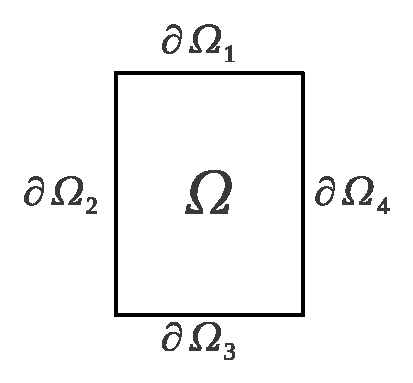
\includegraphics[scale=0.4]{domain}
  \caption{\label{fig:domain} Calculation domain $\Omega\subset\mathbb{R}^2$
  	with boundaries $\partial\Omega_{1\ldots 4}\subset\partial\Omega$.}
  \end{centering}
\end{figure}

The model for solving NPN system is implemented in Hermes2D. In this work
a rectangular 2D domain $\Omega\subset\mathbb{R}^2$ with boundaries 
$\partial\Omega_{1\ldots 4}\subset\partial\Omega$  is considered (see Fig.~\ref{fig:domain}). 
As there is now flow considered in or out of the domain and there is no
constant concentration at the boundaries, zero Neumann boundary conditions are used 
for Eq.~\eqref{eq:nernst-planck}:
\begin{equation}
  -D \frac{\partial C}{\partial n} - z \mu F C \frac{\partial \phi} {\partial n} = 0.
  \label{eq:nernst-planck-boundary}
\end{equation}
As a positive voltage $V_{pos}$ is applied on $\Omega_1$ and $V_{neg}=0$ is applied
on $\Omega_3$, Dirichlet boundary conditions are used for Eq.~\eqref{eq:poisson} for
boundaries $\Omega_1$ and $\Omega_3$:
\begin{eqnarray}
  \phi_{\partial\Omega_1}&=&V_{pos},\\
  \phi_{\partial\Omega_3}&=&0,
  \label{eq:dirichlet}
\end{eqnarray}
and Neumann boundaries for $\Omega_2$ and $\Omega_4$:
\begin{equation}
  \frac{\partial \phi_{\Omega_2}}{\partial n}=\frac{\partial \phi_{\Omega_4}}{\partial n}=0.
\end{equation}


\subsection{Weak form of Poisson-Nernst-Planck system}

To make the derivation of the weak forms more convenient, the following
helper constants will be used: 
\begin{eqnarray}
  K & = &z \mu F,\\
  L&=&\frac{F}{\varepsilon}.
  \label{eq:KL}
\end{eqnarray}
So Eq.~\eqref{eq:nernst-planck} and Eq.~\eqref{eq:poisson} become after 
substituting Eq.~\eqref{eq:rho} and the constants $K$ and $L$:
\begin{eqnarray}
  \frac{\partial C}{\partial t}-D\nabla^2 C-K\nabla\cdot \left(C\nabla\phi\right)&=&0,\label{eq:nernst-planck-2}\\
  -\nabla^2\phi-L\left(C-C_{0}\right)&=&0.\label{eq:poisson-2}
\end{eqnarray}
The boundary condition Eq.~\eqref{eq:nernst-planck-boundary} becomes:
\begin{equation}
  -D\frac{\partial C}{\partial n}-KC\frac{\partial\phi}{\partial n}=0.
  \label{eq:nernst-planck-boundary-2}
\end{equation}
The space for solution is $V=H^1\left(\Omega\right)$ where 
$H^1\left(\Omega\right)=\left\{v\in L^2\left(\Omega\right);\ \nabla v \in \left[L^2\left(\Omega\right)\right]^2\right\}$.
Let's choose a test function $v^C\in V$.
The weak form the Nernst-Planck equation Eq.~\eqref{eq:nernst-planck-2}
is found by multiplying it with the test function $v^C$ and then integrating over the domain~$\Omega$:
\begin{equation}
  \int_{\Omega}\frac{\partial C}{\partial t}v^C d\mathbf{x}
  -\int_{\Omega}D\nabla^2Cv^C d\mathbf{x}-\int_{\Omega}K\nabla C\cdot
  \nabla\phi v^C d\mathbf{x} - \int_{\Omega}KC\nabla^2\phi v^C d\mathbf{x}=0.
  \label{eq:nernst-planck-weak1}
\end{equation}
After adding the weak form of the boundary term 
(Eq.~\eqref{eq:nernst-planck-boundary-2}) and applying
the Green's first identity to the terms that contain Laplacian $\nabla^2$ we get
\begin{eqnarray}
 && \int_{\Omega}\frac{\partial C}{\partial t}v^C d\mathbf{x}+
  D\int_{\Omega}\nabla C\cdot\nabla v^C d\mathbf{x}-
  K\int_{\Omega}\nabla C \cdot \nabla \phi v^C d\mathbf{x}+
  K\int_{\Omega}\nabla\left(Cv^C\right)\cdot \nabla \phi d\mathbf{x}\\
  &&-D\int_{\partial\Omega}\frac{\partial C}{\partial n}v^C d\mathbf{S}-
  \int_{\partial\Omega}K\frac{\partial\phi}{\partial n}Cv^C d\mathbf{S}=0.
  \label{eq:nernst-planck-weak2}
\end{eqnarray}
After expanding the nonlinear term and given that the boundary terms
do not contribute, the weak form becomes
\begin{equation}
  \int_{\Omega}\frac{\partial C}{\partial t}v^C d\mathbf{x}+
  D\int_{\Omega}\nabla C \cdot \nabla v^C d\mathbf{x}-
  K\int_{\Omega}\nabla C \cdot \nabla \phi v^C d\mathbf{x}+
  K\int_{\Omega}\nabla \phi \cdot \nabla C v^C d\mathbf{x}+
  K\int_{\Omega} C \left(\nabla\phi\cdot\nabla v^C\right) d\mathbf{x}=0.
  \label{eq:nernst-planck-weak3}
\end{equation}
As the second and third term cancel out, the final weak from of 
the Nernst-Planck equation is
\begin{equation}
  \int_{\Omega}\frac{\partial C}{\partial t}v^C d\mathbf{x}+
  D\int_{\Omega}\nabla C \cdot \nabla v^C d\mathbf{x}+
  K\int_{\Omega} C \left(\nabla\phi\cdot\nabla v^C\right) d\mathbf{x}=0.
  \label{eq:nernst-planck-weak-final}
\end{equation}
Similarly the weak form of Poisson equation Eq.~\ref{eq:poisson-2}
with a test function $v^\phi\subset V$ is:
\begin{equation}
  -\int_{\Omega}\nabla^2\phi v^\phi d\mathbf{x}-\int_{\Omega}LCv^\phi d\mathbf{x}+
  \int_{\Omega}LC_{0}v^\phi d\mathbf{x}=0.
  \label{eq:poisson-weak1}
\end{equation}
After expanding the $\nabla^2$ terms, the final form becomes
\begin{equation}
  \int_{\Omega}\nabla\phi\cdot\nabla v^\phi d\mathbf{x}-\int_{\Omega}LCv^\phi d\mathbf{x}+
  \int_{\Omega}LC_{0}v^\phi d\mathbf{x}=0.
  \label{eq:poisson-weak-final}
\end{equation}


\subsection{Implementation in Hermes2D}
To implement the system of equations Eq.~\eqref{eq:nernst-planck-weak-final}
and Eq.~\eqref{eq:poisson-weak-final}, the residuals and the Jacobian
matrix must be derived. For that, Crank-Nicolson time stepping was
used
\begin{equation}
  \frac{\partial C}{\partial t} \approx \frac{C^{n+1} - C^n}{\tau},
  \label{eq:cranic}
\end{equation}
where $\tau$ is a time step. For the variables $C^{n+1}$ and $\phi^{n+1}$ the
following notation will be used:
\begin{eqnarray}
  C^{n+1} &=& \sum_{k=1}^{N^C} y_k^{C} v_k^{C}, \label{eq:cnotation}j\\
  \phi^{n+1} &=& \sum_{k=1}^{N^{\phi}} y_k^{\phi} v_k^{\phi}\label{eq:phinotation},
\end{eqnarray}
where $v_k^C$ and $v_k^\phi$ are piecewise polynomial functions in $V$.
Considering the Crank-Nicolson time stepping and the notation~\eqref{eq:cnotation},
the time discretized Eq.~\eqref{eq:nernst-planck-weak-final} becomes
\begin{eqnarray}
  F_i^C\left(Y\right) & = & \int_{\Omega} \frac{C^{n+1}}{\tau}v_i^C d\mathbf{x} - 
  \int_{\Omega} \frac{C^{n}}{\tau}v_i^C d\mathbf{x}\nonumber\\
  &&+\frac 12 \left[D\int_{\Omega} \nabla C^{n+1} \cdot \nabla v_i^C d\mathbf{x}+ 
  	D\int_{\Omega} \nabla C^{n} \cdot \nabla v_i^C d\mathbf{x}\right]\nonumber\\
  &&+ \frac 12 \left[K\int_{\Omega}C^{n+1} \left(\nabla \phi^{n+1} \cdot \nabla v_i^C\right) d\mathbf{x}+
  K\int_{\Omega}C^{n} \left(\nabla \phi^{n} \cdot \nabla v_i^C\right) d\mathbf{x}\right]\label{eq:Fc},
\end{eqnarray}
and in the notation~\eqref{eq:phinotation}, Eq.~\eqref{eq:poisson-weak-final} becomes
\begin{equation}
  F_i^{\phi}\left(Y\right) = \int_{\Omega} \nabla \phi^{n+1} \cdot \nabla v_i^{\phi} d\mathbf{x} 
  - \int_{\Omega} LC^{n+1}v_i^{\phi} d\mathbf{x} + \int_{\Omega} LC_0 v_i^{\phi} d\mathbf{x}.
  \label{eq:Fphi}
\end{equation}
For the implementation the $2\times 2$ Jacobian matrix $DF/DY$ with elements corresponding to
\begin{equation}
  \frac{\partial F_i^C}{\partial y_j^C}, \ \frac{\partial F_i^C}{\partial y_j^{\phi}},\  
  \frac{\partial F_i^{\phi}}{\partial y_j^C}, \ \frac{\partial F_i^{\phi}}{\partial y_j^{\phi}},
\end{equation}
must be derived: 
\begin{eqnarray}
  \frac{\partial F_i^C}{\partial y_j^C} &=& 
  \int_{\Omega} \frac{1}{\tau} v_j^C v_i^C d\mathbf{x} + 
  \frac 12 D\int_{\Omega} \nabla v_j^C \cdot \nabla v_i^C d\mathbf{x}
  + \frac 12 K\int_{\Omega} v_j^C \left(\nabla \phi^{n+1} \cdot \nabla v_i^C\right) d\mathbf{x},\label{eq:dFcdyc}\\
  \frac{\partial F_i^C}{\partial y_j^{\phi}} &=&
  \frac 12 K \int_{\Omega} C^{n+1} \left(\nabla v_j^{\phi} \cdot \nabla v_i^C\right) d\mathbf{x},\\
  \frac{\partial F_i^{\phi}}{\partial y_j^C} &=&
  - \int_{\Omega} L v_j^C v_i^{\phi} d\mathbf{x},\\
  \frac{\partial F_i^{\phi}}{\partial y_j^{\phi}} &=&
  \int_{\Omega} \nabla v_j^{\phi} \cdot \nabla v_i^{\phi} d\mathbf{x}\label{eq:dFphidyphi}.
\end{eqnarray}
In Hermes2D Eq.~\eqref{eq:Fc} and \eqref{eq:Fphi} define the residuum $F$ and
Eq.~\eqref{eq:dFcdyc}---\eqref{eq:dFphidyphi} define the Jacobian matrix $J$.

\subsection{Adaptive multi-mesh solution}

The defined Jacobian $J$ and residuum $F$ can be simply solved in Hermes2D by
using Newton's iteration. However, we were more interested in the automatic
adaptivity and the calculation differences with a single-mesh and multi-mesh.

In case of the single mesh, the same basis function base was used, i.e.
$v_i^\phi=v_i^C$. For multi mesh, the meshes and therefore the basis functions
were different. Regardless of the meshing, automatic adaptivity was applied
during each time step, till the error converged to the acceptable level.
In analogy to the most successful adaptive ODE solvers, Hermes2D uses a pair of 
approximations with different orders of accuracy to obtain this information: 
coarse mesh solution and fine mesh solution. The initial coarse mesh is read 
from the mesh file, and the initial fine mesh is created through its 
global refinement both in $h$ and $p$. For more
information, see~\cite{Hermes-project}. In the calculations, the coarse
mesh solution was not calculated at each time step, but the fine mesh
solution was projected to the coarse mesh by using orthogonal projection. This
yielded better convergence and also faster calculation.

Hermes2D supports 8 different refinement modes, namely,
3 isotropic and 5 anisotropic refinements. The isotropic refinements are
\emph{h}-isotropic (H\_ISO), \emph{p}-isotropic (P\_ISO), \emph{hp}-isotropic (HP\_ISO).
Anisotropic refinement modes are
\emph{h}-anisotropic (H\_ANISO),
\emph{hp}-anisotropic-\emph{h} (HP\_ANISO\_H), \emph{p}-anisotropic (P\_ANISO),
\emph{hp}-anisotropic-p (HP\_ANISO\_P), and \emph{hp}-anisotropic (HP\_ANISO).
Once the refinement mode is selected (by user), Hermes2D selects a particular
refinement scheme from several candiates based on the score. More information
can be found in~\cite{Hermes-project}.


